\documentclass[11pt,a4paper]{article}
\usepackage[utf8]{inputenc}
\usepackage[spanish]{babel}
\usepackage{graphicx}
\usepackage{pdfpages} % Paquete fundamental para insertar el PDF de la carátula
\usepackage{float}
\usepackage{geometry}
\geometry{top=2.5cm, bottom=2.5cm, left=2.5cm, right=2.5cm}

\begin{document}

% Inserta la carátula ocupando toda la primera hoja
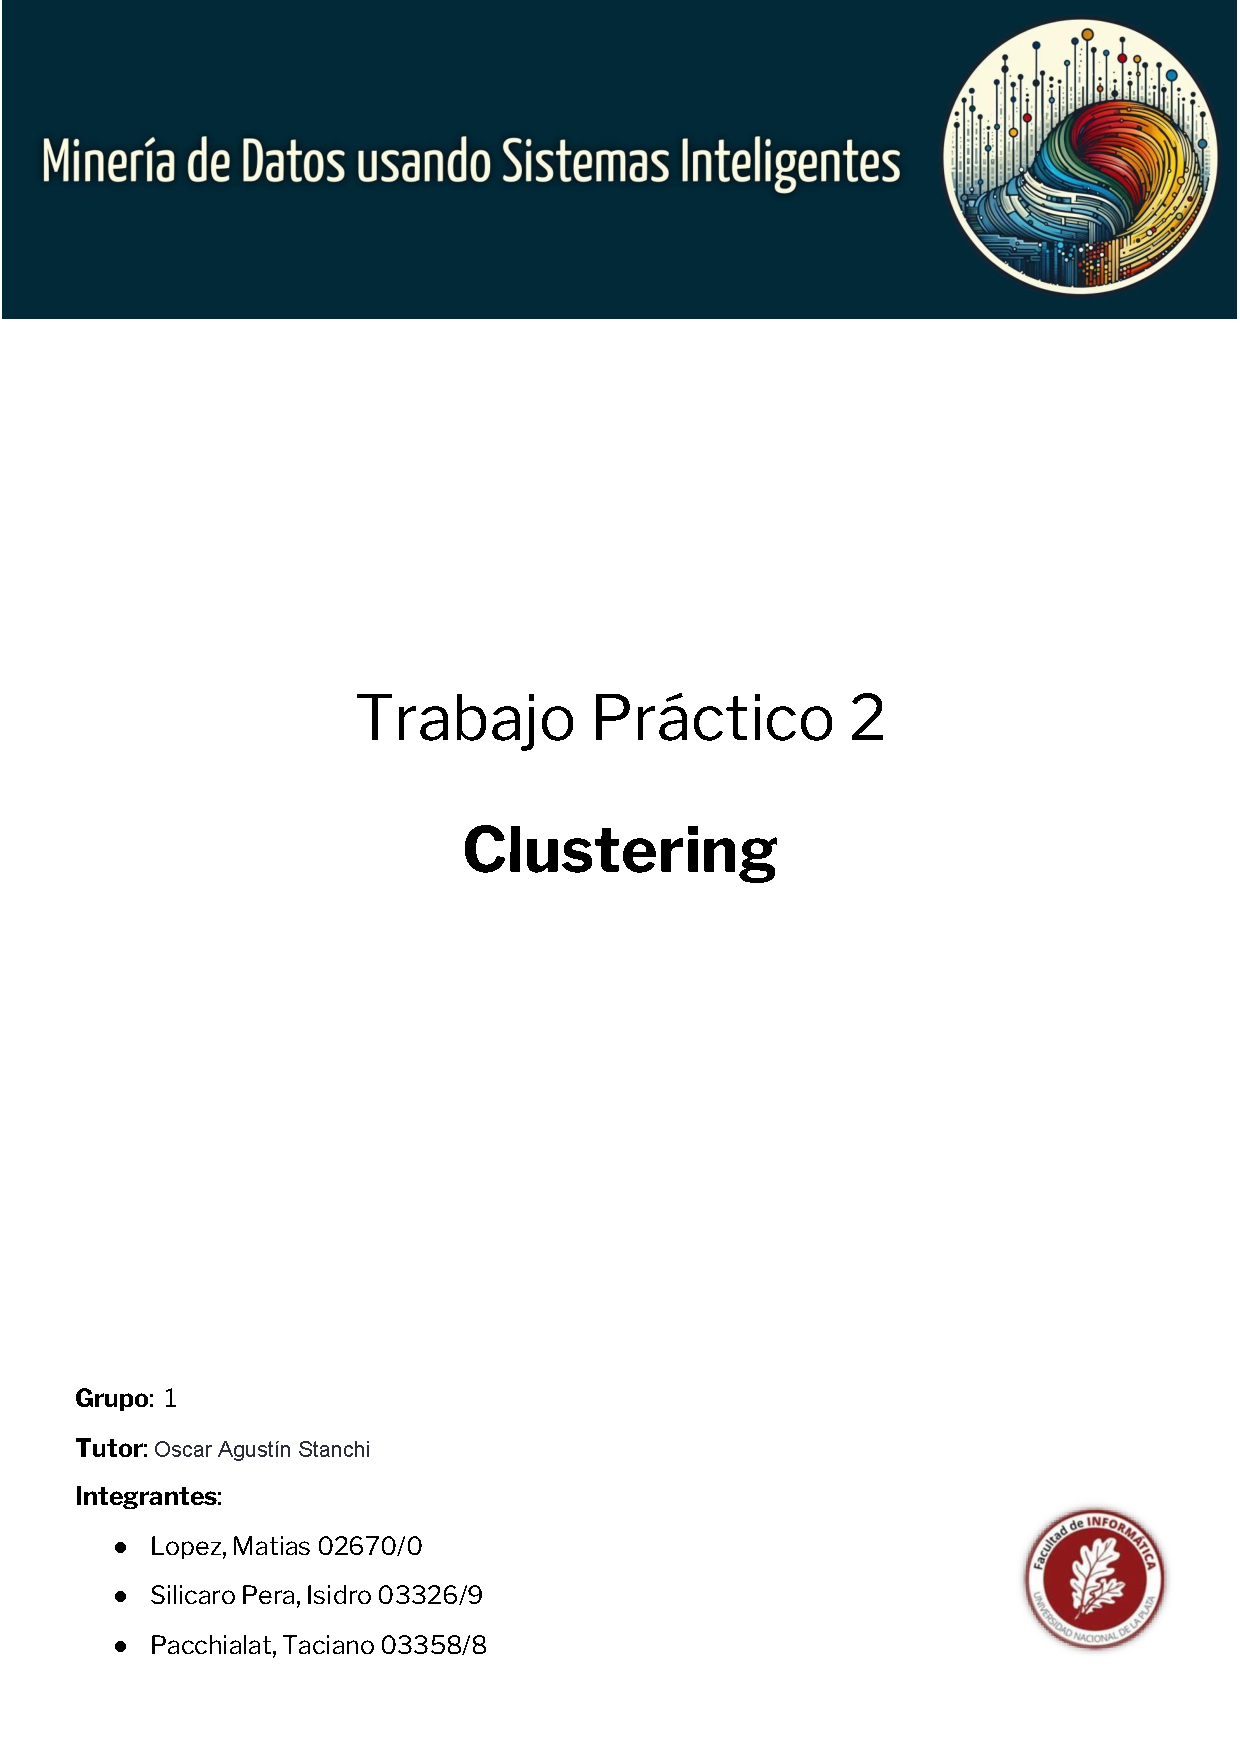
\includepdf[pages={1}]{imagenes/Caratula_para_entrega2.pdf}

\section*{2. Algoritmo K-medias}

\subsection*{Inciso A}
En la siguiente figura se ilustran las posiciones iniciales de los datos ($x_1, x_2, x_3, x_4$) y los centroides ($c_1, c_2$) en el plano X-Y.

\begin{figure}[H]
    \centering
    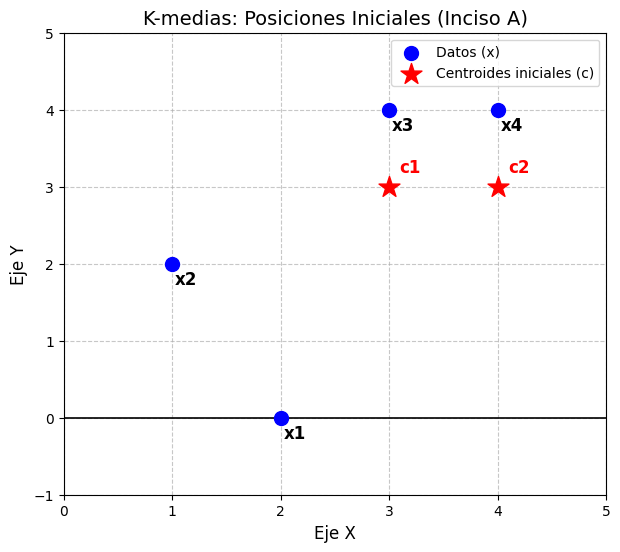
\includegraphics[width=0.7\textwidth]{imagenes/incisoA.png}
    \caption{Posiciones iniciales de datos y centroides.}
\end{figure}

\vspace{1cm}

\subsection*{Inciso B}
A continuación, se presenta la tabla con los resultados finales tras realizar tres iteraciones del algoritmo K-medias con $k=2$, utilizando la distancia euclídea al cuadrado.

\begin{figure}[H]
    \centering
    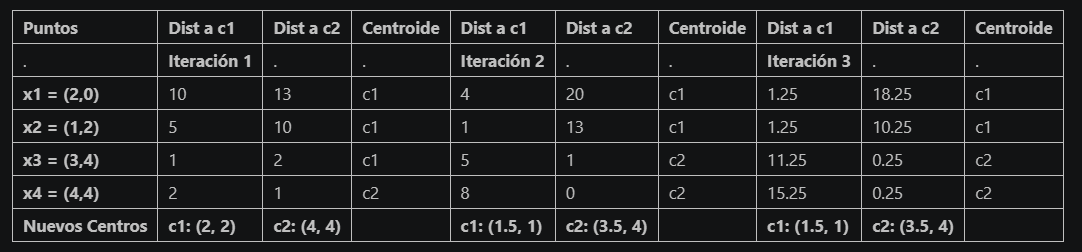
\includegraphics[width=\textwidth]{imagenes/IncisoB.png}
    \caption{Tabla de resultados de las iteraciones de K-medias.}
\end{figure}

\newpage
\subsection*{Anexo: Cálculos de cada inciso}
En las siguientes imágenes se adjuntan los cálculos desarrollados a mano correspondientes a las asignaciones de distancias y actualización de centroides para cada iteración.

\begin{figure}[H]
    \centering
    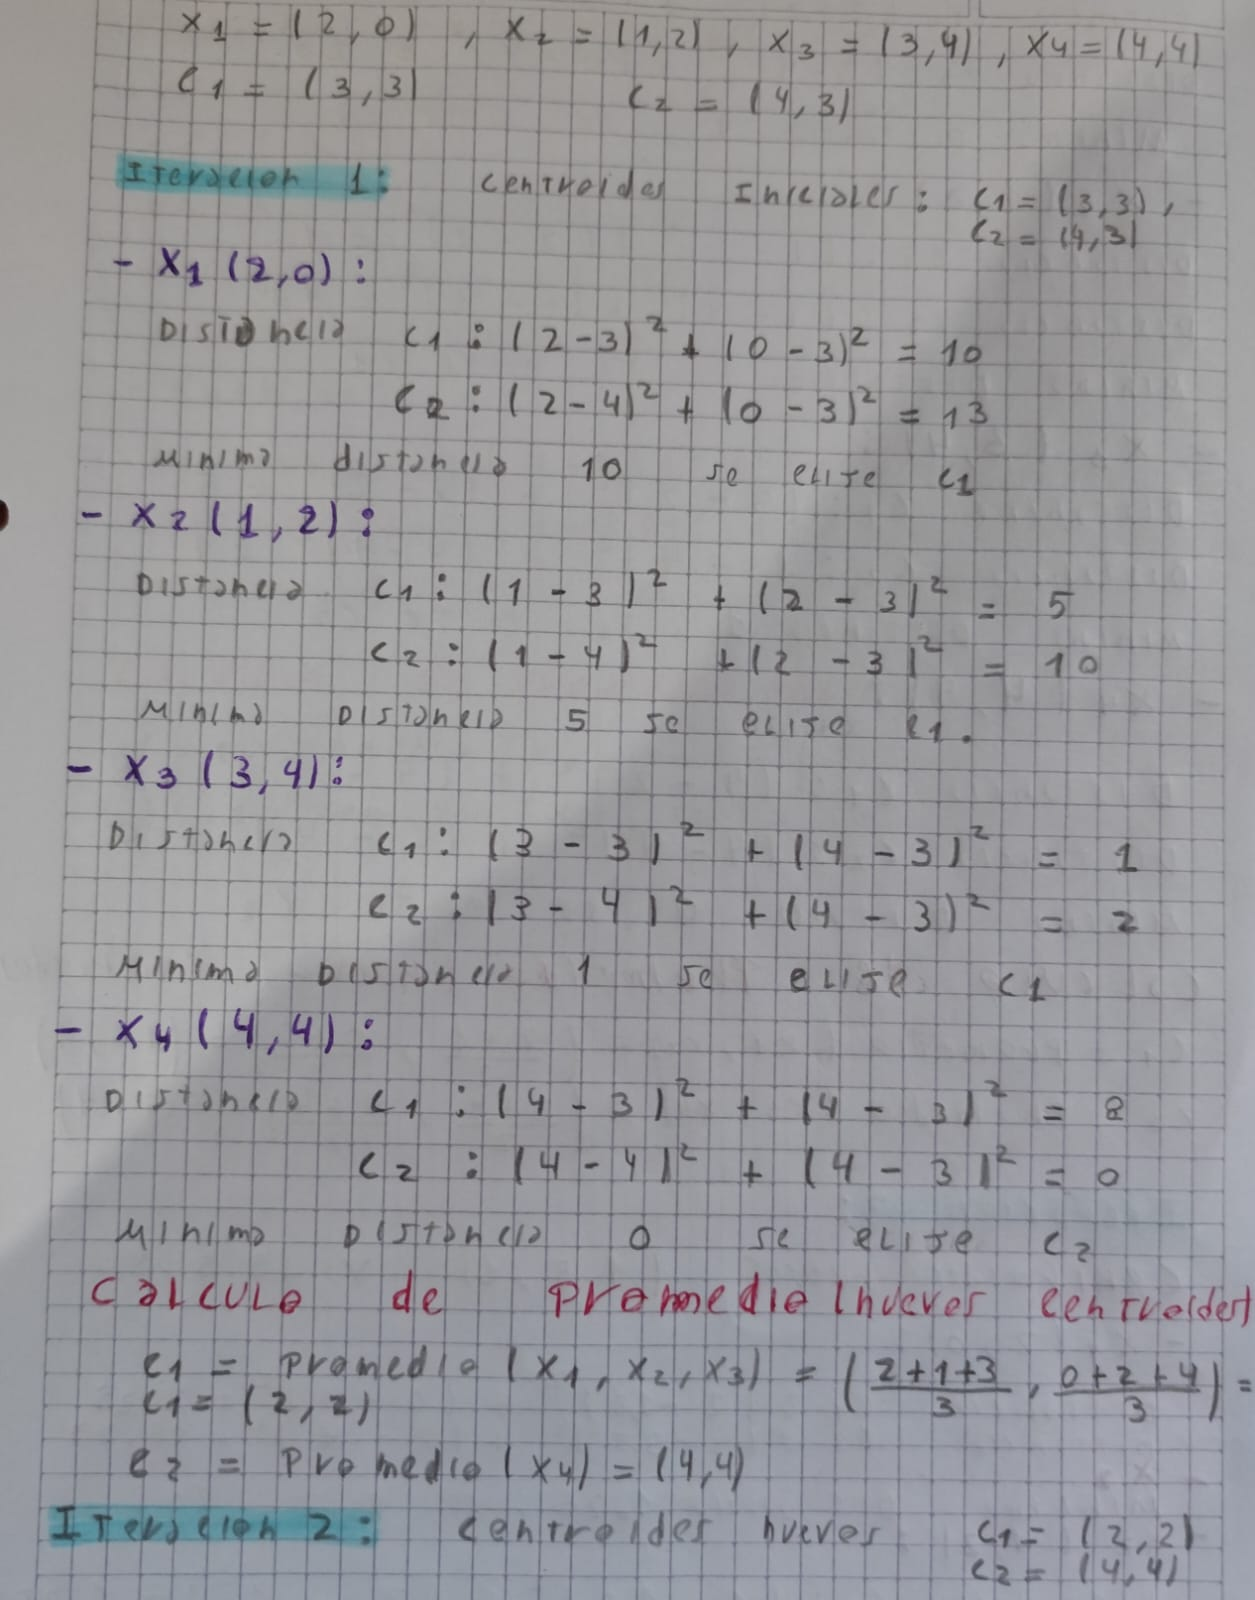
\includegraphics[width=0.8\textwidth]{imagenes/IncisoB1.jpeg}
    \caption{Cálculos a mano - Parte 1.}
\end{figure}

\begin{figure}[H]
    \centering
    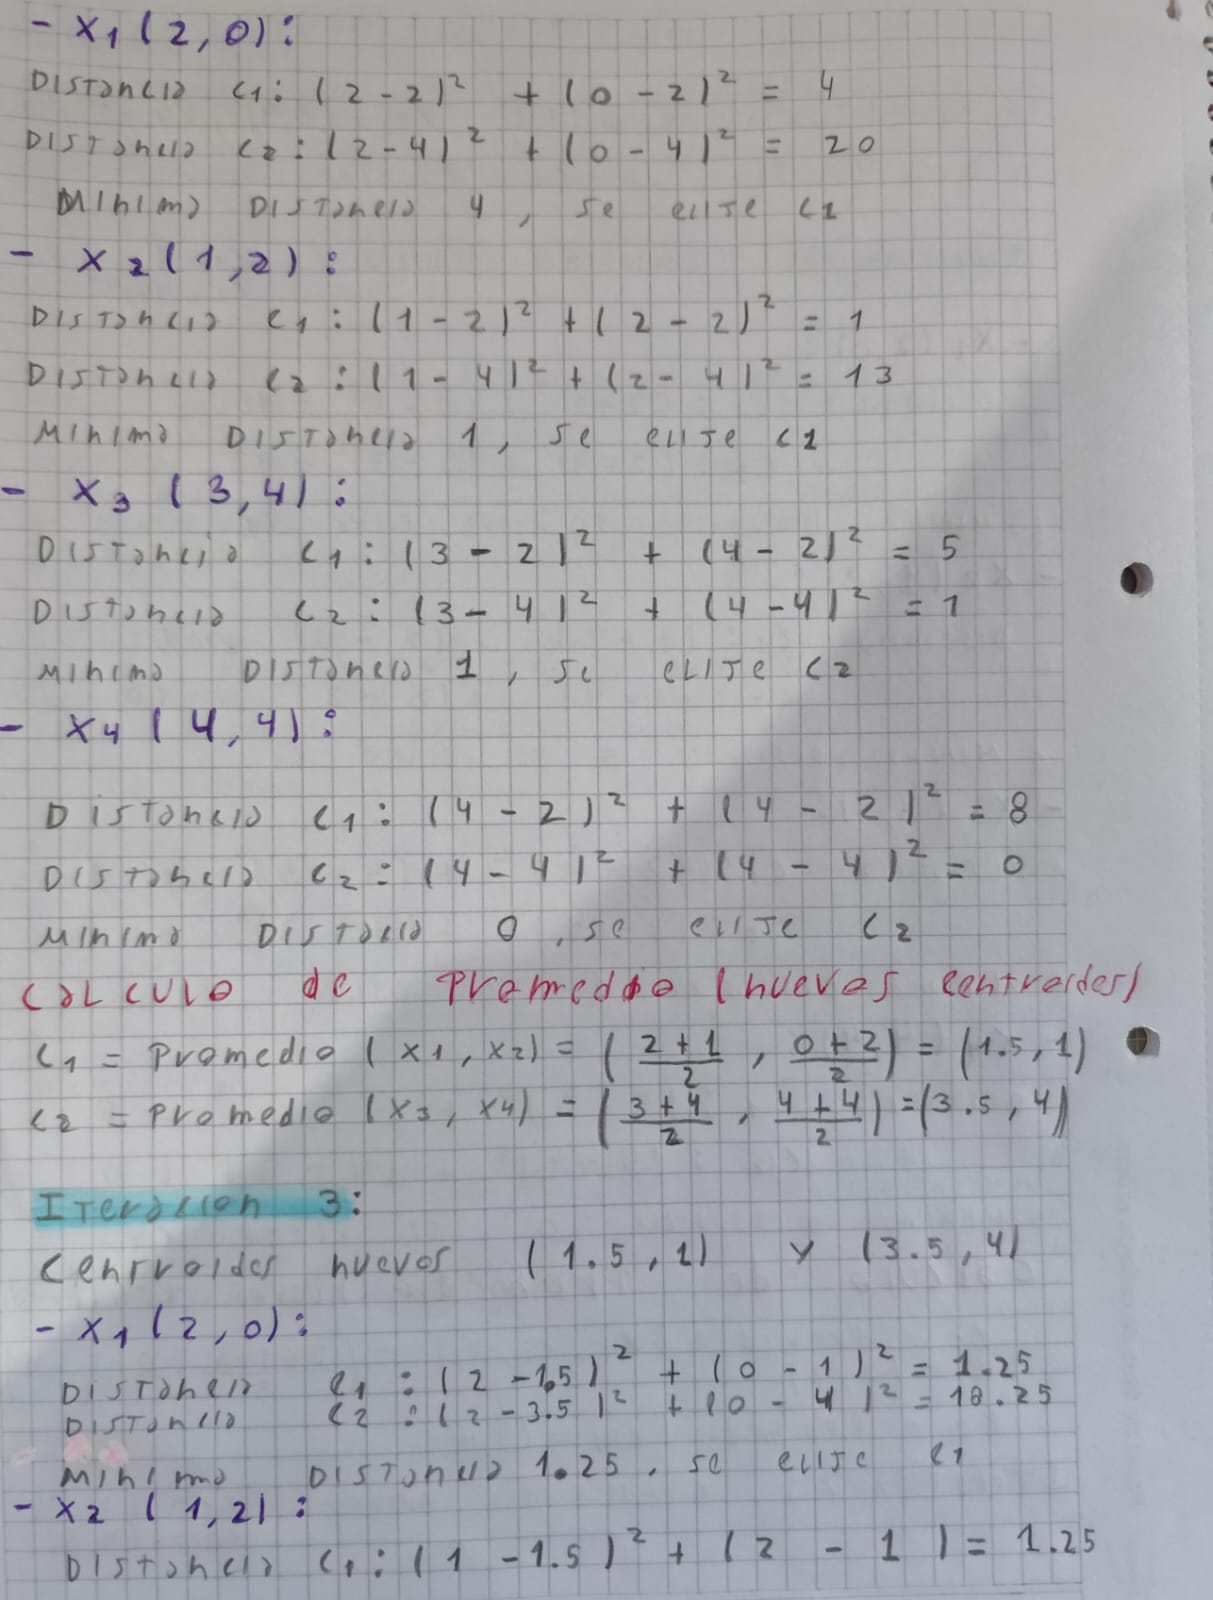
\includegraphics[width=0.8\textwidth]{imagenes/IncisoB2.jpeg}
    \caption{Cálculos a mano - Parte 2.}
\end{figure}

\begin{figure}[H]
    \centering
    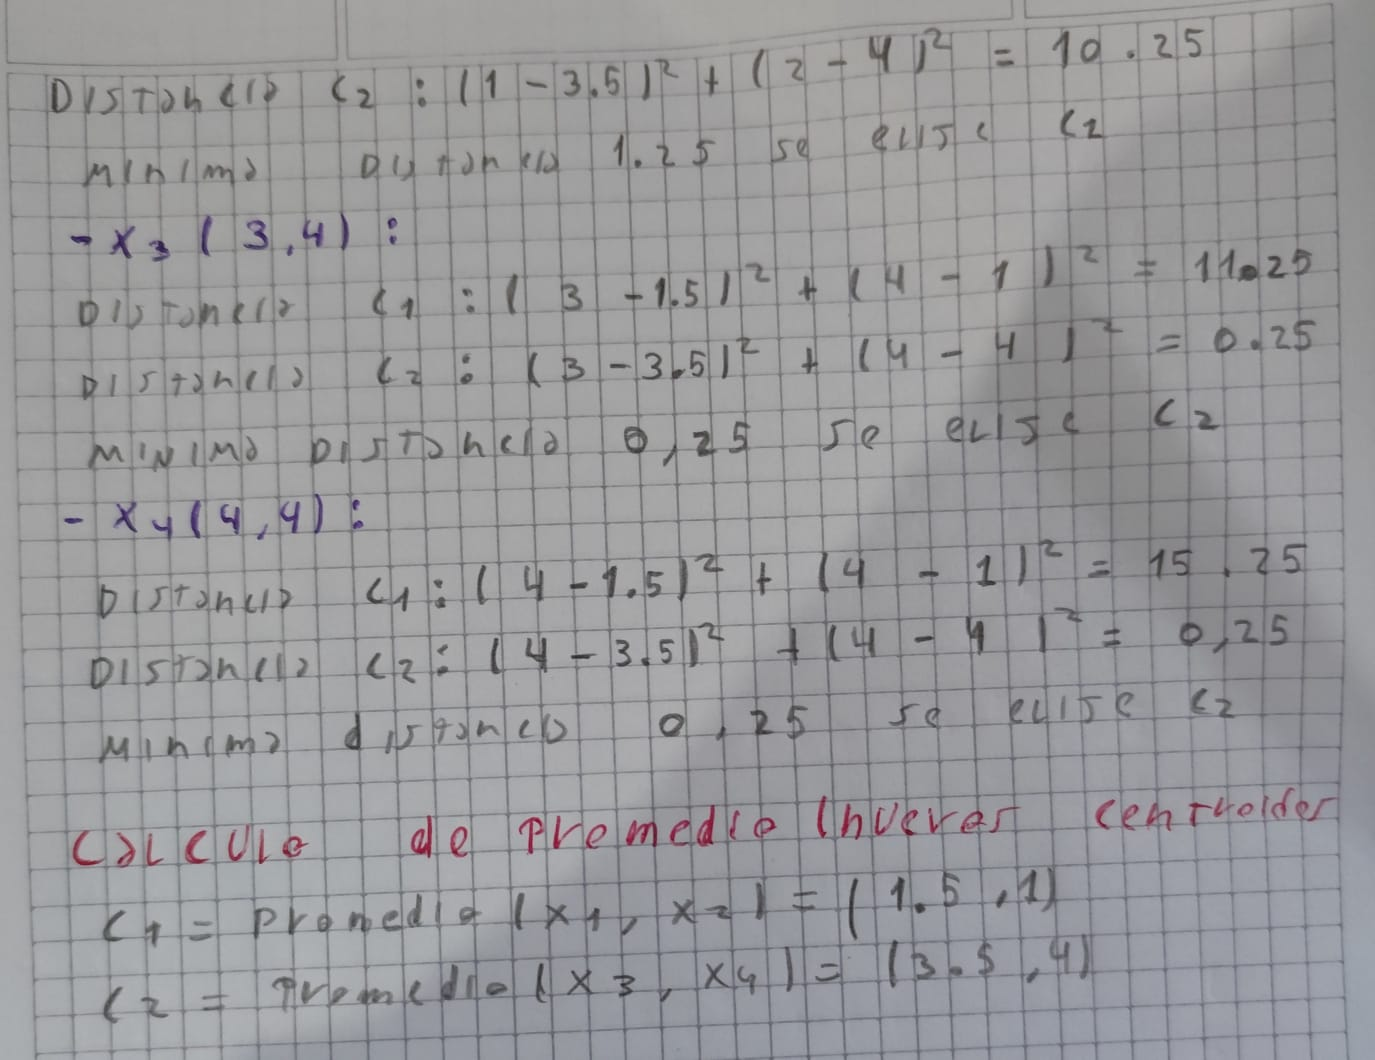
\includegraphics[width=0.8\textwidth]{imagenes/IncisoB3.jpeg}
    \caption{Cálculos a mano - Parte 3.}
\end{figure}

\end{document}